\documentclass{beamer}
\usepackage{tikz}

\usetikzlibrary{positioning}
\usetheme{Darmstadt}

\begin{document}

\section{Structure of the compiler}
\begin{frame}{Main ideas}
	\begin{figure}
		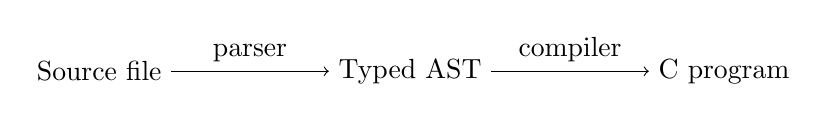
\begin{tikzpicture}
			\node (sf) {Source file};
			\node[right =2cm of sf] (ast) {Typed AST};
			\node[right =2cm of ast] (C) {C program};
			\draw
				(sf) edge[->] node[above] {parser} (ast)
				(ast) edge[->] node[above] {compiler} (C);
		\end{tikzpicture}
		\caption{Structure of the compiler}
	\end{figure}
\end{frame}

\begin{frame}{Testing}
	\begin{block}{Passes}
		The passes can be split into:
		\begin{itemize}
			\item those checking the program validity
			\item those modifying the AST of the program
		\end{itemize}
	\end{block}
\end{frame}

\section{Typed AST}
\subsection{First attempt using GADTs}
\begin{frame}
	\begin{block}{Main idea}
		Using GADTs to represent nodes and expressions allows to ensure the
		well-typedness of a program.
	\end{block}
	\begin{figure}
		\centering
		\includegraphics[width=.75\textwidth]{imgs/gadt.png}
	\end{figure}
\end{frame}
\begin{frame}
	\begin{block}{Pros of using GADTs}
		\begin{itemize}
			\item Any term of the GADT represents a well-typed program
			\item Extending the language to support more types consists of adding
				constructors to variables and constants
			\item The types are easy to read and understand
		\end{itemize}
	\end {block}

	\begin{block}{Cons of using GADTs}
		\begin{itemize}
			\item
			They cannot be dynamically generated (hence it is impossible to
			implement a parser that gives back a GADT)
			\item
			One should think about the isomorphism between
			\texttt{a $\ast$ (b $\ast$ c)} and \texttt{(a $\ast$ b) $\ast$ c}.
		\end{itemize}
	\end{block}
\end{frame}

\subsection{Second attempt: using explicit types in the variables, expressions,
\dots{} constructors}
\begin{frame}
	\begin{block}{Idea}
		Explicitly collect typing information while parsing.
	\end{block}
	\begin{figure}
		\centering
		\includegraphics[width=.6\textwidth]{imgs/explicit_types.png}
	\end{figure}
\end{frame}

\begin{frame}
	\begin{block}{Pros of using explicit types}
		\begin{itemize}
			\item Programs can be built dynamically, hence a parser can be
			written
			\item While parsing, the parser has all the required information on
			the sub-variables/nodes/expressions to check the well-typedness
		\end{itemize}
	\end{block}
	\begin{block}{Cons of these definitions}
		\begin{itemize}
			\item The typing information on terms is very redundant.
			\item The rejection of ill-typed programs depends on the correctness
			of the parser
		\end{itemize}
	\end{block}
\end{frame}

\section{Passes}
\begin{frame}{Passes}
	\begin{block}{Classification}
		The passes of our compiler are functions of taking a program and either:
		\begin{itemize}
			\item returning a program if the pass succeeded
			\item returns nothing otherwise
		\end{itemize}

		We only have one language in our compiler: no intermediary language.
	\end{block}
\end{frame}

\subsection{Check}
\begin{frame}
	\begin{block}{Passes}
		The passes can be split into:
		\begin{itemize}
			\item those checking the program validity
			\item those modifying the AST of the program
		\end{itemize}
	\end{block}
\end{frame}

\begin{frame}{Implemented passes}
	\begin{block}{\texttt{pre}-propagation to leaves}
	\end{block}
	\begin{block}{Check: unique initialization for variables}
	\end{block}
	\begin{block}{Linearization of the equations}
	\end{block}
\end{frame}

\end{document}

